% =============================================================
%  SECTION 7, Integrated MD Engine
% ============================================================

\section{Integrated MD Engine}

\subsection{Putting It All Together}

"Each of the six modules was independently built and tested before being integrated into a single working simulation. The core engine is implemented as a single Python class, \texttt{MDSimulation}. This class maintains the complete simulation state, including positions, velocities, forces, and the Verlet neighbour list, and orchestrates the execution of each module in the correct sequence.

\subsection{How the Modules Connect}

The simulation is executed in three distinct phases: initialisation, an equilibration loop, and a production loop. While Figure~\ref{fig:md_flowchart} maps the high-level data routing between modules, the specific physical constraints and parameters applied during each phase are detailed below.

\begin{figure}[H]
\centering
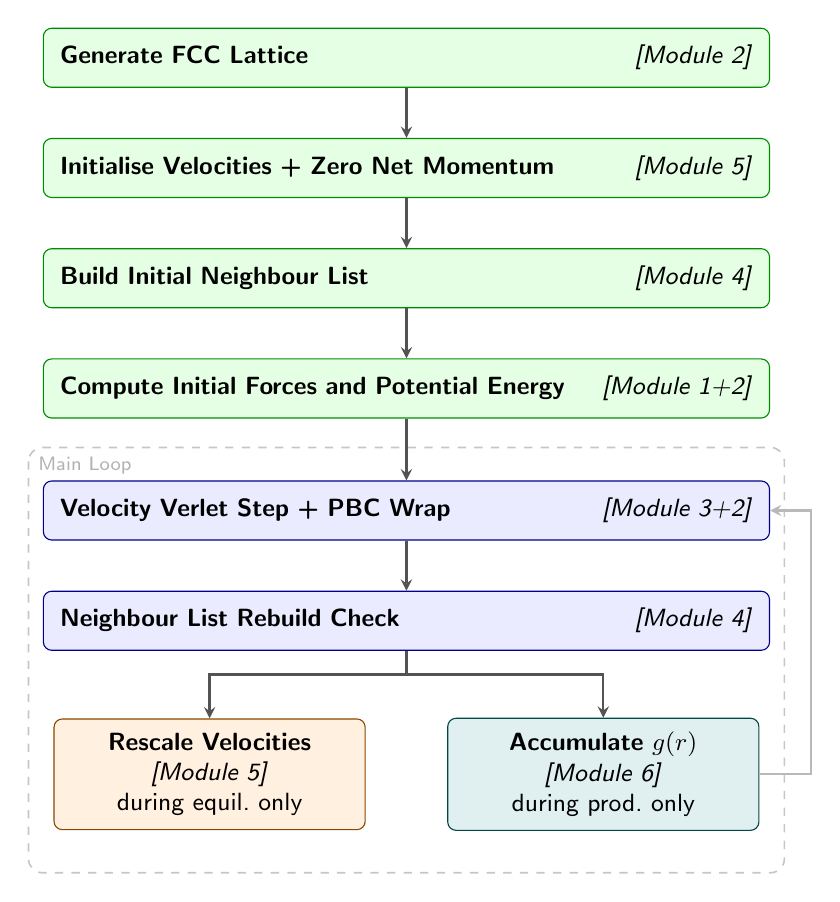
\begin{tikzpicture}[
    ibox/.style = {
        draw, rounded corners=3pt,
        fill=green!10, draw=green!55!black,
        text width=8.8cm, minimum height=0.75cm,
        align=left, inner sep=6pt, font=\small\sffamily
    },
    lbox/.style = {
        draw, rounded corners=3pt,
        fill=blue!8, draw=blue!55!black,
        text width=8.8cm, minimum height=0.75cm,
        align=left, inner sep=6pt, font=\small\sffamily
    },
    ebox/.style = {
        draw, rounded corners=3pt,
        fill=orange!12, draw=orange!55!black,
        text width=3.6cm, minimum height=1.4cm,
        align=center, inner sep=5pt, font=\small\sffamily
    },
    pbox/.style = {
        draw, rounded corners=3pt,
        fill=teal!12, draw=teal!55!black,
        text width=3.6cm, minimum height=1.4cm,
        align=center, inner sep=5pt, font=\small\sffamily
    },
    arr/.style = {->, thick, >=stealth, color=gray!65!black}
]

%% ---- INITIALISATION ----
\node[ibox] (fcc)  at (0,  0.0) {\textbf{Generate FCC Lattice} \hfill \textit{[Module 2]}};
\node[ibox] (vel)  at (0, -1.4) {\textbf{Initialise Velocities + Zero Net Momentum} \hfill \textit{[Module 5]}};
\node[ibox] (nb0)  at (0, -2.8) {\textbf{Build Initial Neighbour List} \hfill \textit{[Module 4]}};
\node[ibox] (f0)   at (0, -4.2) {\textbf{Compute Initial Forces and Potential Energy} \hfill \textit{[Module 1+2]}};

%% ---- LOOP BORDER ----
\draw[dashed, gray!45, rounded corners=5pt, line width=0.6pt]
    (-4.8, -4.95) rectangle (4.8, -10.35);
\node[font=\scriptsize\sffamily, color=gray!60, anchor=north west]
    at (-4.8, -4.95) {Main Loop};

%% ---- LOOP NODES ----
\node[lbox] (vv)      at (0, -5.75) {\textbf{Velocity Verlet Step + PBC Wrap} \hfill \textit{[Module 3+2]}};
\node[lbox] (rebuild) at (0, -7.15) {\textbf{Neighbour List Rebuild Check} \hfill \textit{[Module 4]}};

%% ---- BRANCH NODES ----
\node[ebox] (rescale) at (-2.5, -9.1)
    {\textbf{Rescale Velocities}\\\textit{[Module 5]}\\during equil.\ only};
\node[pbox] (rdf)     at ( 2.5, -9.1)
    {\textbf{Accumulate $g(r)$}\\\textit{[Module 6]}\\during prod.\ only};

%% ---- ARROWS ----
\draw[arr] (fcc.south)     -- (vel.north);
\draw[arr] (vel.south)     -- (nb0.north);
\draw[arr] (nb0.south)     -- (f0.north);
\draw[arr] (f0.south)      -- (vv.north);

\draw[arr] (vv.south)      -- (rebuild.north);
\draw[arr] (rebuild.south) -- ++(0,-0.3) -| (rescale.north);
\draw[arr] (rebuild.south) -- ++(0,-0.3) -| (rdf.north);

\draw[arr, color=gray!55]
    (rdf.east) -- ++(0.65, 0) |- (vv.east);

\end{tikzpicture}
\caption{Data flow through the integrated MD engine. \textbf{Green} boxes run once at the start. \textbf{Blue} boxes run every time step. \textbf{Orange} (velocity rescaling) is on only during equilibration; \textbf{teal} ($g(r)$ sampling) is on only during production. The right side arrow shows the loop repeating back to the Verlet step.}
\label{fig:md_flowchart}
\end{figure}
\begin{description}
    \item[Initialisation (Runs Once):] Establishes the starting state. The box length $L^*$ is derived from the target density $\rho^*$ or the lattice parameter $a$, and atoms are placed on an FCC lattice. Initial velocities are drawn from a Maxwell-Boltzmann distribution, with the centre-of-mass velocity explicitly subtracted to ensure zero net momentum. Finally, the baseline neighbour list, Lennard-Jones forces, and potential energies are computed to bootstrap the integrator.

    \item[Equilibration ($N_{\text{equil}}$ steps):] Drives the system toward the target temperature $T^*_{\text{target}}$. Positions and velocities are integrated via Velocity Verlet, with periodic boundaries strictly enforced via modulo arithmetic during the position update. The neighbour list is dynamically rebuilt only if an atom's displacement exceeds half the skin distance. To force thermalization\footnote{While thermalization broadly describes a physical system relaxing toward thermal equilibrium, in this context it specifically refers to the algorithmic process of rescaling atomic velocities to drive and maintain the system at the target reduced temperature, $T^*$.}, velocities are rescaled every \texttt{rescale\_interval} (10 steps in this work). No structural data is collected during this phase.

    \item[Production (NVE Ensemble):] Simulates the natural, unforced dynamics of the system. The velocity rescaling thermostat is disabled to strictly conserve energy (NVE ensemble). Instead, the algorithm focuses on data collection, sampling the radial distribution function $g(r)$ every \texttt{rdf\_interval} steps for subsequent time-averaging and structural analysis.
\end{description}

To execute the full melting sweep, this entire three-stage pipeline is re-initialized and executed for each individual temperature point.

\subsection{The Velocity Verlet Kernel}

The core of both loops is \texttt{\_verlet\_step}, which runs the full four step Velocity Verlet algorithm in four lines:

\begin{lstlisting}[caption={The integration kernel in \texttt{md\_engine.py}. All four lines implement Equations~\eqref{eq:vv_pos} to \eqref{eq:vv_vfull} directly. The \texttt{\% L} on line 2 applies the PBC wrap in the same operation as the position update.}, label={lst:vv_kernel}]
def _verlet_step(self, pos, vel, f, L, nb):
    pos_new = (pos + vel*self.dt + 0.5*f*self.dt**2) % L  # step 1 + PBC
    v_mid   =  vel + 0.5*f*self.dt                         # step 2
    pe, f_new = self._calculate_forces(pos_new, nb, L)     # step 3
    return pos_new, v_mid + 0.5*f_new*self.dt, pe, f_new  # step 4
\end{lstlisting}

Line 2 is worth a closer look: the modulo operator \texttt{\% L} wraps atoms back into the box in the same line as the position update; there is no separate PBC call, and it handles arbitrarily large displacements correctly. Line 4 uses the forces at the \emph{new} positions to complete the velocity update. 

\subsection{Main Loop Architecture}

As the simulation framework was scaled to accommodate comprehensive temperature sweeps and diagnostic tracking, the core execution loop was abstracted into a parallelized architecture. The listing below presents a high-level structural map of the \texttt{MDSimulation} execution flow, highlighting how the modules interact within a given worker process.

\begin{lstlisting}[language=Python, caption={High-level architectural map of the integrated MD execution flow. The main thread distributes the workload, while individual worker processes handle the time integration and data collection for each temperature point.}, label={lst:main_loop}]
# 1. Parallel Task Manager (Main Thread)
def run(self):
    pos0, L = self.generate_fcc_lattice()
    
    # Delegate each temperature run to a parallel worker process
    results = pool.map(self._run_one_temperature, worker_args)
    return results

# 2. Core Worker Function (Executes per T*)
def _run_one_temperature(args):
    # ===================== INITIALISATION ===========================
    pos, vel, force, nb_list = bootstrap_system_state(args)
    pos_ref = pos.copy()
    
    # ===================== EQUILIBRATION ============================
    for step in range(equil_steps):
        pos, vel, pe, force = verlet_step(pos, vel, force, nb_list)
        
        # Rebuild neighbour list if any atom drifted too far
        if needs_rebuild(pos, pos_ref):
            nb_list = update_neighbor_list(pos)
            pos_ref = pos.copy()
            
        # Rescale velocities to force target temperature
        if step % rescale_interval == 0:
            vel = rescale_velocities(vel, T_star)
            
        record_diagnostics(kin_E, pot_E, momentum)

    # ===================== PRODUCTION ===============================
    for step in range(prod_steps):
        pos, vel, pe, force = verlet_step(pos, vel, force, nb_list)
        
        if needs_rebuild(pos, pos_ref):
            nb_list = update_neighbor_list(pos)
            pos_ref = pos.copy()
            
        record_diagnostics(kin_E, pot_E, momentum)
        
        # Sample structural data (Thermostat is OFF)
        if step % rdf_interval == 0:
            accumulate_rdf(pos)

    return time_averaged_rdf, diagnostic_traces
\end{lstlisting}

The main \texttt{run()} method optimizes execution by using a multiprocessing pool to evaluate multiple reduced temperatures ($T^*$) concurrently. Each worker process isolates the system state and handles two main phases: equilibration and production. 

Two key features define this execution loop:
\begin{itemize}
    \item \textbf{Dynamic Neighbour Lists:} The simulation tracks atomic displacements from a reference state (\texttt{pos\_ref}). The neighbour list is only rebuilt when an atom moves further than $\delta_\text{skin}/2$, guaranteeing accurate force calculations with minimal computational overhead.
    \item \textbf{Diagnostic Tracking:} Kinetic energy, potential energy, and net momentum are recorded at every step to verify numerical stability and ensure energy conservation during the microcanonical (NVE) production phase.
\end{itemize} 
\newpage

\subsection{Simulation Parameters}

Table~\ref{tab:integrated_params} lists the parameters used throughout the project. The system ($n_\text{cells} = 4$, $N = 256$) was used for all Krypton properties, diagnostics, and melting runs. The full source code is in \texttt{md\_engine.py}, which accompanies this report.

\begin{table}[H]
    \centering
    \caption{MD engine parameters.}
    \label{tab:integrated_params}
    \begin{tabular}{llc}
        \toprule
        \textbf{Parameter} & \textbf{Symbol} & \textbf{Value} \\
        \midrule
        Unit cells per side      & $n_\text{cells}$                  & 4       \\
        Total atoms              & $N = 4\,n_\text{cells}^3$         & 256     \\
        Reduced density          & $\rho^*$                          & 0.8442  \\
        Box length               & $L^* = (N/\rho^*)^{1/3}$          & 6.718   \\
        Time step                & $\delta t^*$                      & 0.005   \\
        Cutoff radius            & $r_c^*$                           & 2.5     \\
        Skin radius              & $r_s^*$                           & 3.0     \\
        Rebuild threshold        & $(r_s^* - r_c^*)/2$               & 0.25    \\
        Equilibration steps      & $N_\text{equil}$                  & 2000    \\
        Production steps         & $N_\text{prod}$                   & 2000    \\
        Rescale interval         & steps between rescaling           & 10      \\
        $g(r)$ sample interval   & steps between RDF frames          & 10      \\
        $g(r)$ frames averaged   & $N_\text{prod} / \text{interval}$ & 200     \\
        RDF bins                 & $n_b$                             & 200     \\
        \bottomrule
    \end{tabular}
\end{table}

